\documentclass[../main.tex]{subfiles}

\begin{document}

\chapter[Decomposing the Model Predictive Control]{Decomposing the\\ Model Predictive Control}
\epigraph{\centering The mystery of the universe \\ is not time \\but size.}
{\textit{The Gunslinger}\\\textsc{Stephen King}}

\minitoc

In this chapter we present the Model Predictive Control strategy and we present some considerations needed to decompose it.

\section{Model Predictive Control}
Model Predictive Control, or even \mpc, is a closed-loop control strategy based
on the solution of optimization problems.
Given a system model and an objective function, this strategy uses the system model to predict future states and compute a control sequence that optimizes the given objective function.
Since the solution is found by using optimization problems, it is natural to add some restrictions on the system, which are usually defined as (in)equality constraints.

The fact that constraints can be easily added to the specifications gave it a special place in the industry, where is largely used in a plethora of applications (\todo{add uses of MPC in the industry}).

\subsection{General discrete \mpc\ }
As it is generally implemented through a digital computer and the transmission of continuous signals can potentially demand infinite bandwidth~\cite{HeEtAl2022}, it is natural to assume the system to be modeled with discrete-time dynamics
\begin{equation}
\vec{x}[k+1]=f(\vec{x}[k],\vec{u}[k]),
\end{equation}
where $\vec{x}[k]:\R^{n_{x}}$ is the state of the system and $\vec{u}[k]:\R^{n_{u}}$ is the input of the system.

The system can be under constraints
\begin{equation}
 h(\vec{x}[k],\vec{u}[k])\preceq\0,
\end{equation}
with $h:\R^{n_{x}}\times\R^{n_{u}}\to\R^{n_{c}}$. Observe that mathematically equality constraints can be represented by a couple of inequality constraints, although for implementation in computers it can lead to poor numerical conditioning, resulting unexpected behavior~\cite{BorrelliEtAl2017}.

Given an objective function $J:\R^{n_{x}}\times\R^{N\cdot n_{u}}\to \R$, we can optimize this objective for a given horizon $\set{H}=\{1\mathbin{:}N\}$ to obtain a control sequence $\vec{U}[k]=[\vec{u}[k|k]\T \dots \vec{u}[k+N-1|k]\T]$, where
we use states and input predictions of time $k+i$ calculated in a time $k$, represented by $\vec{x}[k+i|k]$ and $\vec{u}[k+i|k]$. The problem solved to calculate the control sequence is

\begin{equation}\label{eq:general_mpc}
  \small
  \begin{aligned}
    \begin{matrix}
      \underset{\vec{U}[k]}{\mathrm{minimize}} & J(\vec{x}[k|k],\vec{U}[k])&\\
      \mathrm{subject~ to} &

      \left.  \begin{aligned}
          \quad \vec{x}[k+i|k]=f(\vec{x}[k+i-1|k],\vec{u}[k+i-1|k])\\
          \quad                h(\vec{x}[k+i-1|k],\vec{u}[k+i-1])\preceq\0
        \end{aligned}\qquad        \right\}

      \begin{aligned}
        \forall i\in\set{H}
      \end{aligned}
    \end{matrix}
  \end{aligned}
\end{equation}
After solving this problem, we have an optimal control sequence $\vec{U}^{\star}[k]$ and only the first element $\vec{u}^{\star}[k|k]$ is applied in the system. The process is repeated for $k+1$ following a \rhs.

This formulation is as general as possible, but depending on the problem's convexity it can be hard to solve it, specially online.
Convex problems are the most widely studied, and strategies to solve them are extensively diffused. Some of those problems even have explicit solutions~\cite{BoydVandenberghe2004}.

\subsection{Convex \mpc\ (quadratic case) }
The \mpc\ community favors the use of convex problems when possible. Two families of convex problems broadly used are \qp\ and \lp.
In this work we concentrate on \qp\ problems, whose objective functions are quadratic and constraints are affine or linear. Numerous mathematical solvers are apt to solve this kind of problem directly or through equivalent problems. We can cite non-extensivily some solvers such as MATLAB internal QP solvers\footnote{\url{https://fr.mathworks.com/help/optim/ug/quadprog.html}}, OSQP\footnote{\url{https://osqp.org}}, MOSEK\footnote{\url{https://www.mosek.com}} and ECOS\footnote{\url{https://github.com/embotech/ecos}}.

A commonly quadratic objective function used is
\begin{equation}
  \label{eq:quadratic_objective_with_sum}
  J(\vec{x}[k|k],\vec{U}[k])=\sum_{i\in\set{H}}\left[\norm{\mpcvec{v}[ ][k+i][k]}^{2}_{Q} +\norm{\mpcvec{u}[ ][k+i-1][k]}^{2}_{R}\right]
\end{equation}
where $\vec{v}$ is a control objective, and ${ Q:\semidefpos }$ and ${ R:\defpos }$ are weighting matrices, which can represent costs of each term of the equation. The relation between these matrices describe the compromise between control signal energy and control objective.

The control objectives can be for example, \emph{disturbance rejection}, where ${ \vec{v}[k]=\vec{x}[k] }$, or \emph{reference tracking}, where ${ \vec{v}[k]=\vec{w}[k]-\vec{x}[k] }$, being $\vec{w}[k]$ a setpoint.
Observe that this last example is for state reference tracking, for output reference tracking the system output $\vec{y}[k]$ should be used instead of $\vec{x}[k]$, depending on the system an adequate relation between $\vec{y}[k]$ and $\vec{x}[k]$ can be found.

The predictions of $\vec{v}[k]$ and $\vec{w}[k]$ can be stacked as ${ \vec{V}[k]=[\vec{v}[k+1|k]\T \dots \vec{v}[k+N|k]\T] }$ and
${ \vec{W}[k]=[\vec{w}[k+1|k]\T \dots \vec{w}[k+N|k]\T] }$ and then~\eqref{eq:quadratic_objective_with_sum} can be rewritten as
\begin{equation}
  \label{eq:quadratic_objective_compact}
  J(\vec{x}[k|k],\vec{U}[k])=\norm{\vec{V}[k]}^{2}_{\bar{Q}} + \norm{\vec{U}[k] }^{2}_{\bar{R}},
\end{equation}
where $\bar{Q}=\kron{I_{N}}{Q}$ and
$\bar{R}=\kron{I_{N}}{R}$.

For the constraints in~\eqref{eq:general_mpc} to be affine or linear, first we suppose the system is linear and we use a linear time-invariant model
\begin{equation}\label{eq:large_scale_system_model}
  \begin{array}{rl}
    \vec{x}[k+1]&=A\vec{x}[k]+B\vec{u}[k]\\
    \vec{y}[k]&=C\vec{x}[k]
  \end{array}
.
\end{equation}
In this work we concentrate in input constraint systems whose constraints do no depend on the system state, so we drop the $\vec{x}[k]$ terms in $h$, and since it is affine or linear we rewrite it as
\begin{equation}
  \Gamma\vec{u}[k]\preceq\vec{u}_{\max}
\end{equation}
which can be vectorized for an horizon in $\mathcal{H}$
\begin{equation}
\bar{\Gamma}\vec{U}[k]\preceq {\vec{U}}_{\text{max}},
\end{equation}
with ${ \bar{\Gamma}=\kron{I_{N}}{\Gamma} }$ and ${ \vec{U}_{\max}=\kron{\1_{N}}{\vec{u_{max}}} }$.

For the control objectives, henceforth we only consider \emph{reference tracking}, since \emph{disturbance rejection} can be described as a \emph{reference tracking} when ${ C=I_{n_{x}} }$ and ${ \vec{w}[k]=\0_{n_{x}} }$.

Putting it all together we have
\begin{equation}
  \small
  \begin{aligned}
    \begin{matrix}
      \underset{\vec{U}[k]}{\mathrm{minimize}} &\norm{\vec{V}[k]}^{2}_{\bar{Q}} + \norm{\vec{U}[k] }^{2}_{\bar{R}}&\\
      \mathrm{subject~ to} &
      \vec{x}[k+i|k]=A\vec{x}[k+i-1|k]+B\vec{u}[k+i-1|k]
      &
       \forall i\in\set{H} \\
      &\bar{\Gamma}\vec{U}[k]\preceq {\vec{U}}_{\text{max}}&

    \end{matrix}
  \end{aligned}
  \label{eq:general_qp}
  \quad.
\end{equation}

If we opt for a Batch Approach~\cite[Chapter 8.2]{BorrelliEtAl2017} to solve the problem, we can rewrite the equalities in~\eqref{eq:general_qp} compactly as
% cite:BorrelliEtAl2017 pag188
\begin{equation}
    \begin{matrix}
      \underbrace{
        \left[
          \begin{matrix}
            \vec{y}[k+1|k] \\
            \vec{y}[k+2|k] \\
            \vdots \\
            \vec{y}[k+N|k]
          \end{matrix}
        \right]
      }_{\vec{Y}[k]} &=&
      \underbrace{
        \left[
          \begin{matrix}
            CA^{1} \\
            CA^{2} \\
            \vdots \\
            CA^{N}
          \end{matrix}
        \right]
      }_{\mathcal{Y}^{x}}
      \vec{x}[k|k]+
      \underbrace{
        \left[
          \begin{matrix}
            CA^{0}B & 0 & \dots & 0 \\
            CA^{1}B& \ddots & \ddots & \vdots      \\
            \vdots     & \ddots   & \ddots & \vdots    \\
            CA^{N-1}B & \dots & \dots & CA^{0}B
          \end{matrix}
        \right]
      }_{\mathcal{Y}^{u}}
      \vec{U}[k]
    \end{matrix}
    \quad .
\end{equation}
and substitute them in the objective function, yielding the \qp\ problem which implicitly respects these constraints
\begin{equation}
  \label{eq:quadratic_objective_compact_batch}
  \begin{aligned}
    \begin{matrix}
      \underset{\vec{U}[k]}{\mathrm{minimize}} &
      \norm{\vec{U}[k]}^{2}_{H} + 2{\vec{f}[k]}^{T}\vec{U}[k] + c[k] &\\
      \mathrm{subject~ to} &
\bar{\Gamma}\vec{U}[k]\preceq {\vec{U}}_{\text{max}}
    \end{matrix}
  \end{aligned}
\end{equation}

where
\begin{equation}
\begin{array}{lll}
H&=&\norm{\mathcal{Y}^{u}}^{2}_{\bar{Q}}+\bar{R}\\
\vec{f}[k]&=&{\mathcal{Y}^{u}}^{T}\bar{Q}(\mathcal{Y}^{x}\vec{x}[k|k]-\vec{W}[k])\\
c[k]&=&\norm{\mathcal{Y}^{x}\vec{x}[k|k]}^{2}_{\bar{Q}}-2{\vec{W}[k]}^{T}\bar{Q}{\mathcal{Y}^{x}}\vec{x}[k|k]+\norm{\vec{W}[k]}^{2}_{\bar{Q}}
\end{array}.
\end{equation}
By dividing the objective function by $2$ and ignoring the constant term $c[k]$ we have a problem structured in the standard \qp\ form which can be easily used in the solvers supracited
\begin{equation}
  \label{eq:qp_standard_form}
  \begin{aligned}
    \begin{matrix}
      \underset{\vec{U}[k]}{\mathrm{minimize}} &
      \frac{1}{2}\norm{\vec{U}[k]}^{2}_{H} + {\vec{f}[k]}^{T}\vec{U}[k] &\\
      \mathrm{subject~ to} &
\bar{\Gamma}\vec{U}[k]\preceq {\vec{U}}_{\text{max}}
    \end{matrix}
  \end{aligned}.
\end{equation}
Observe that even if the problem in \eqref{eq:qp_standard_form} is equivalent (same solution) to the one in~\eqref{eq:quadratic_objective_compact_batch}, they are not the same problem, so we still need to recalculate the function in~\eqref{eq:quadratic_objective_compact_batch} using the optimal $\vec{U}^{\star}[k]$ found to obtain the correct objective function value.

Although the solution of such problems can be straightforward, since solvers are widely known and the problem is well structured, it can be computationally intensive depending on the sizes of $n_{x}$, $n_{u}$ and $N$.
For large-scale systems such as \todo{(add 2/3 examples)}, the computation time and memory needed to solve their associated problems increase drastically.
Some decomposition methods can be used to make the solution of such problems more tractable, using different time-scales (\todo[hierarchical dmpc in ChristofidesEtAl2013, Abreu talvez??]{Citation?}) for instance.
In this work we will focus on decomposition techniques based on optimization decomposition.

\section{Optimization Decomposition Frameworks}
\label{sec:decomp-fram}
In this section we briefly describe the optimization decomposition frameworks finding what they have in common so we can decompose the \mpc\ problem proposed.
As seen in~\cite{BoydVandenberghe2004}, maximization problems can be rewritten as minimization problems so we use only minimization problems henceforth.
\subsection{Decomposable problems}\label{sec:decomposable_problems}
As shown in~\cite{ConejoEtAl2006} and~\cite{BoydEtAl2015}, a decomposable optimization problem has more than 1 decision variable and can be decomposed into at least 2 sub-problems.
For simplicity, the examples given in this section divide problems into 2 sub-problems.
If the sub-problems variables can also be partitioned, we can partition the original problem even further.

% \begin{remark}
The examples in this section are decomposed using the primal problem which is the most direct method, other methods exist and will be shortly commented during this work.
% \end{remark}

Be the following problem a general decomposable problem, i.e., the decision variable $\vec{x}$ can be partitioned into two groups of variables $\vec{x}_{1}$ and $\vec{x}_{2}$:
\begin{equation}\label{eq:general_decomposable_optimization_problem}
  \small
  \begin{aligned}
    \begin{matrix}
      \underset{\vec{x}_{1},\vec{x}_{2}}{\mathrm{minimize}}  &J(\vec{x}_{1},\vec{x}_{2})&\\
      \mathrm{subject~ to} &

           f_{i}(\vec{x}_{1},\vec{x}_{2}) \leq 0 \text{, } i\in\set{M}=\{1\mathbin{:}m\}\\
          & g_{i}(\vec{x}_{1},\vec{x}_{2}) = 0\text{, } i\in\set{P}=\{1\mathbin{:}p\}\\
    \end{matrix}
  \end{aligned}
\end{equation}

Such family of problems can be divided into two categories:
\begin{enumerate}
  \item Uncoupled
  \item Coupled
\end{enumerate}

\subsection{Uncoupled problems}\label{sec:uncoupled_problems}
The decomposition of uncoupled problems is straightforward and trivial, being so rare in the real world that it is frequently ignored.

 For an uncoupled problem, the groups of variables $\vec{x}_{1}$ and $\vec{x}_{2}$ are disjoint, the function $J(\vec{x})$ can be rewritten  as $J(\vec{x})=J_{1}(\vec{x}_{1})+J_{2}(\vec{x}_{2})$, and the constraints can be divided into $2$ groups, one that depends only on $\vec{x}_{1}$ and other only on $\vec{x}_{2}$, i.e. $\set{M}_{1}$ and $\set{M}_{2}$ for the inequality constraints and $\set{P}_{1}$ and $\set{P}_{2}$ for the equality ones:
\begin{equation}\label{eq:general_uncoupled_optimization_problem}
  \small
  \begin{aligned}
    \begin{matrix}
      \underset{\vec{x}_{1},\vec{x}_{2}}{\mathrm{minimize}}  &J_{1}(\vec{x}_{1})&+&J_{2}(\vec{x}_{2})&\\
      \mathrm{subject~ to} &

           f_{i}(\vec{x}_{1}) \leq 0 \text{, } i\in\set{M}_{1}& & f_{i}(\vec{x}_{2}) \leq 0 \text{, } i\in\set{M}_{2}\\
          & g_{i}(\vec{x}_{1}) = 0\text{, } i\in\set{P}_{1}& & g_{i}(\vec{x}_{2}) = 0\text{, } i\in\set{P}_{2}\\
    \end{matrix}
  \end{aligned}.
\end{equation}

We can trivially rewrite~\eqref{eq:general_uncoupled_optimization_problem} as
\begin{equation}\label{eq:general_uncoupled_optimization_problem_main_problem}
  \small
  \begin{aligned}
    \begin{matrix}
      \underset{\vec{x}_{1},\vec{x}_{2}}{\mathrm{minimize}}  &{J_{1}(\vec{x}_{1}^{\star})}+{J_{2}(\vec{x}_{2}^{\star})}
    \end{matrix}
  \end{aligned},
\end{equation}
where ${J_{1}(\vec{x}_{1}^{\star})}$ and ${J_{2}(\vec{x}_{2}^{\star})}$ can be found by solving
\begin{subequations}\label{eq:general_uncoupled_optimization_problem_decomposed}
\begin{equation}\label{eq:general_uncoupled_optimization_problem_decomposed_1}
    {J_{1}(\vec{x}_{1}^{\star})}=\begin{matrix}
      \underset{\vec{x}_{1}}{\mathrm{minimize}}  &J_{1}(\vec{x}_{1})\\
      \mathrm{subject~ to} &

           f_{i}(\vec{x}_{1}) \leq 0 \text{, } i\in\set{M}_{1}\\
          & g_{i}(\vec{x}_{1}) = 0\text{, } i\in\set{P}_{1}\\
    \end{matrix}
\end{equation}
\begin{equation}\label{eq:general_uncoupled_optimization_problem_decomposed_2}
    {J_{2}(\vec{x}_{2}^{\star})}=\begin{matrix}
      \underset{\vec{x}_{2}}{\mathrm{minimize}}  &J_{2}(\vec{x}_{2})\\
      \mathrm{subject~ to} &

           f_{i}(\vec{x}_{2}) \leq 0 \text{, } i\in\set{M}_{2}\\
          & g_{i}(\vec{x}_{2}) = 0\text{, } i\in\set{P}_{2}\\
    \end{matrix}
\end{equation}
\end{subequations}
Each problem in~\eqref{eq:general_uncoupled_optimization_problem_decomposed} can be solved in parallel and when solutions $\vec{x}_{i}^{*}$ are found for each sub-problem, the problem in~\eqref{eq:general_uncoupled_optimization_problem_main_problem} is automatically solved ($J_{i}(\vec{x}_{i}^{\star})$ are constants).

\subsection{Coupled problems}
On the other hand, coupled problems are more frequent in the real world.
In this category, the sub-problems can not be entirely solved in parallel since the coupling implies an exchange of information between sup-problems (one sub-problem needs information of other sub-problem to solve itself).
The coupling nature of the problem can be traced to two main sources
\begin{enumerate}
  \item Complicating variables
  \item Complicating constraints
\end{enumerate}
We called them \emph{complicating} because without them the solution would be trivial (uncoupled category shown in the last section)~\cite{ConejoEtAl2006}.

\subsubsection{Complicating variables}
For this sub-category, we suppose the variables $\vec{x}_{1}$ and $\vec{x}_{2}$ are not disjoint, there is some variables in common.
To force disjointedness, we redivided $\vec{x}$ into $3$ disjoint groups $\vec{x}_{a}$ (present only in sub-problem $1$), $\vec{x}_{b}$ (present only in sub-problem $2$), and $\vec{x}_{ab}$ (present in both sub-problems).
We suppose $J(\vec{x})$ can be rewritten  as ${J(\vec{x})=J_{1}(\vec{x}_{a},\vec{x}_{ab})+J_{2}(\vec{x}_{b},\vec{x}_{ab})}$, and the constraints can be divided into groups that depend on $\vec{x}_{a}$ and $\vec{x}_{b}$, i.e. $\set{M}_{a}$ and $\set{M}_{b}$ for the inequality constraints and $\set{P}_{a}$ and $\set{P}_{b}$ for the equality ones:
\begin{equation}\label{eq:general_complicating_variables_optimization_problem}
  \small
  \begin{aligned}
    \begin{matrix}
      \underset{\vec{x}_{a},\vec{x}_{ab},\vec{x}_{b}}{\mathrm{minimize}}  &J_{1}(\vec{x}_{a},\vec{x}_{ab})&+&J_{2}(\vec{x}_{b},\vec{x}_{ab})&\\
      \mathrm{subject~ to} &

      f_{i}(\vec{x}_{a}) \leq 0 \text{, } i\in\set{M}_{a} & & f_{i}(\vec{x}_{b}) \leq 0 \text{, } i\in\set{M}_{b}\\
      & g_{i}(\vec{x}_{a}) = 0\text{, } i\in\set{P}_{a}& & g_{i}(\vec{x}_{b}) = 0\text{, } i\in\set{P}_{b}\\
    \end{matrix}
  \end{aligned}.
\end{equation}

Similarly, we can rewrite~\eqref{eq:general_complicating_variables_optimization_problem} as
\begin{equation}\label{eq:general_complicating_variables_optimization_main_problem}
  \small
  \begin{aligned}
    \begin{matrix}
      \underset{\vec{x}_{a},\vec{x}_{ab},\vec{x}_{b}}{\mathrm{minimize}}  &J_{1}(\vec{x}_{a}^{\star},\vec{x}_{ab})+{J_{2}(\vec{x}_{b}^{\star},\vec{x}_{ab})}
    \end{matrix}
  \end{aligned},
\end{equation}
where $J_{1}(\vec{x}_{a}^{\star},\vec{x}_{ab})$ and $J_{2}(\vec{x}_{b}^{\star},\vec{x}_{ab})$ can be found by solving
\begin{subequations}\label{eq:general_complicating_variables_optimization_problem_decomposed}
\begin{equation}\label{eq:general_complicating_variables_optimization_problem_decomposed_1}
    J_{1}(\vec{x}_{a}^{\star},\vec{x}_{ab})=\begin{matrix}
      \underset{\vec{x}_{a}}{\mathrm{minimize}}  &J_{1}(\vec{x}_{a},\vec{x}_{ab})&\\
      \mathrm{subject~ to} &

           f_{i}(\vec{x}_{a}) \leq 0 \text{, } &i\in\set{M}_{a}\\
          & g_{i}(\vec{x}_{a}) = 0\text{, } &i\in\set{P}_{a}\\
    \end{matrix}
\end{equation}
\begin{equation}\label{eq:general_complicating_variables_optimization_problem_decomposed_2}
    J_{2}(\vec{x}_{b}^{\star},\vec{x}_{ab})=\begin{matrix}
      \underset{\vec{x}_{b}}{\mathrm{minimize}}  &J_{2}(\vec{x}_{b},\vec{x}_{ab})&\\
      \mathrm{subject~ to} &

           f_{i}(\vec{x}_{b}) \leq 0 \text{, } &i\in\set{M}_{b}\\
          & g_{j}(\vec{x}_{b}) = 0\text{, } &j\in\set{P}_{b}\\
    \end{matrix}
\end{equation}
\end{subequations}
Observe that the solutions of~\eqref{eq:general_complicating_variables_optimization_problem_decomposed} depend on a given value of $\vec{x}_{ab}$, thus a coordination between sub-problems is needed to find an optimal $\vec{x}_{ab}^{\star}$ to solve problem~\eqref{eq:general_complicating_variables_optimization_main_problem} and thus the original problem~\eqref{eq:general_complicating_variables_optimization_problem}.

\subsubsection{Complicating Constraints}

For complicating constraints, as the name suggests, instead of variables we have constraints which prevent complete separation into sub-problems.

The variables $\vec{x}_{1}$ and $\vec{x}_{2}$ are disjoint, $J(\vec{x})$ can be rewritten as ${J(\vec{x})=J_{1}(\vec{x}_{1})+J_{2}(\vec{x}_{2})}$ and besides the constraints in sets $\set{M}_{1}$ $\set{M}_{2}$ and $\set{P}_{1}$ $\set{P}_{2}$ we also have equality and inequality constraints which couple $\vec{x}_{1}$ and $\vec{x}_{2}$, denoted ${h_{i}(\vec{x}_{1},\vec{x}_{2})=h_{i_{1}}(\vec{x}_{1})+h_{i_{2}}(\vec{x}_{2}) \leq 0\text{, }i\in\set{O}}$
and ${w_{i}(\vec{x}_{1},\vec{x}_{2})=w_{i_{1}}(\vec{x}_{1})+w_{i_{2}}(\vec{x}_{2}) =0\text{, }i\in\set{N}}$:

\begin{equation}\label{eq:general_complicating_constraints_optimization_problem}
  \small
  \begin{aligned}
    \begin{matrix}
      \underset{\vec{x}_{1},\vec{x}_{2}}{\mathrm{minimize}}  &J_{1}(\vec{x}_{1})&+&J_{2}(\vec{x}_{2})&\\
      \mathrm{subject~ to} &

           f_{i}(\vec{x}_{1}) \leq 0 \text{, } i\in\set{M}_{1}& & f_{i}(\vec{x}_{2}) \leq 0 \text{, } i\in\set{M}_{2}\\
          & g_{i}(\vec{x}_{1}) = 0\text{, } i\in\set{P}_{1}& & g_{i}(\vec{x}_{2}) = 0\text{, } i\in\set{P}_{2}\\
          && h_{i_{1}}(\vec{x}_{1})+h_{i_{2}}(\vec{x}_{2}) \leq 0\text{, } i\in\set{O}\\
          &&w_{i_{1}}(\vec{x}_{1})+w_{i_{2}}(\vec{x}_{2}) = 0\text{, }  i\in\set{N}

    \end{matrix}
  \end{aligned}
\end{equation}
Adding auxiliary variables $\vec{\theta}_{o}$ and $\vec{\theta}_{n}$ we can rewrite the problem as
\begin{equation}\label{eq:general_complicating_constraints_optimization_main_problem}
  \small
  \begin{aligned}
    \begin{matrix}
      \underset{\vec{x}_{1},\vec{x}_{2},\vec{\theta_{o}},\vec{\theta}_{n}}{\mathrm{minimize}}  &J_{1}(\vec{x}_{1}^{\star},\vec{\theta}_{o},\vec{\theta}_{n})+J_{2}(\vec{x}_{2}^{\star},\vec{\theta}_{o},\vec{\theta}_{n})
    \end{matrix}
  \end{aligned},
\end{equation}

where $J_{1}(\vec{x}_{1}^{\star},\vec{\theta}_{o},\vec{\theta}_{n})$ and $J_{2}(\vec{x}_{2}^{\star},\vec{\theta}_{o},\vec{\theta}_{n})$ can be found by solving
\begin{subequations}\label{eq:general_complicating_constraints_optimization_problem_decomposed}
  \begin{equation}
    J_{1}(\vec{x}_{1}^{\star},\vec{\theta}_{o},\vec{\theta}_{n})=\begin{matrix}
      \underset{\vec{x}_{a}}{\mathrm{minimize}}  &&J_{1}(\vec{x}_{1})&\\
      \mathrm{subject~ to} &
      f_{i}(\vec{x}_{a}) \leq 0 \text{, } i\in\set{M}_{1} & & h_{m_{1}}(\vec{x}_{1}) \leq \vec{\theta}_{o}\text{, } m\in\set{O}\\
      & g_{j}(\vec{x}_{a}) = 0\text{, } j\in\set{P}_{1} & & w_{n_{1}}(\vec{x}_{1}) = \vec{\theta}_{n} \text{, }  i\in\set{N}
    \end{matrix}
  \end{equation}\label{eq:general_complicating_constraints_optimization_problem_decomposed_1}%
  \begin{equation}
    J_{2}(\vec{x}_{2}^{\star},\vec{\theta}_{o},\vec{\theta}_{n})=\begin{matrix}
      \underset{\vec{x}_{b}}{\mathrm{minimize}}  &&J_{2}(\vec{x}_{2})&\\
      \mathrm{subject~ to} &
      f_{i}(\vec{x}_{b}) \leq 0 \text{, } i\in\set{M}_{2} & & \hspace{-1em}h_{m_{2}}(\vec{x}_{2}) \leq -\vec{\theta}_{o}\text{, } m\in\set{O}\\
      & g_{j}(\vec{x}_{b}) = 0\text{, } j\in\set{P}_{2} & & \hspace{-1em}w_{n_{2}}(\vec{x}_{2}) = -\vec{\theta}_{n} \text{, }  i\in\set{N}
    \end{matrix}
  \end{equation}\label{eq:general_complicating_constraints_optimization_problem_decomposed_2}%
\end{subequations}

Again, observe that the solutions of~\eqref{eq:general_complicating_constraints_optimization_problem_decomposed} depend on the values of $\vec{\theta}_{o}$ and $\vec{\theta}_{n}$, thus a coordination between sub-problems is needed to find their optimal values in order to solve problem~\eqref{eq:general_complicating_constraints_optimization_main_problem} and thus the original problem~\eqref{eq:general_complicating_constraints_optimization_problem}.

% This is the base of the methodology used in this work to decompose the \mpc, we will re-discuss the method and present examples of implementation in a further section (\todo[add primal decomposition section number]{\S??}).
\begin{remark}
  As seen in~\cite{BoydEtAl2015}, a complicating constraint problem can be transformed into a complicating variable problem and vice versa by the use of auxiliary variables.
  For instance, we can substitute a complicating variable by two new local variables (one for each sub-problem) and add equality constraints to each sub-problem to force them to be equal.
  We will use henceforth only complicating constraints.
\end{remark}

\subsection{Generalizing}
If we observe all the examples given, we can see a pattern emerge:

A problem
\begin{equation}\label{eq:general_coupled_optimization_problem}
  \small
  \begin{aligned}
    \begin{matrix}
      \underset{\text{decision variables}}{\mathrm{minimize}}  &\text{objective}_{1}&+&\text{objective}_{2}&\\
      \mathrm{subject~ to} & \text{constraints}_{1},&&  \text{constraints}_{2}\\
      &&\text{coupling constraints}_{12}&
    \end{matrix}
  \end{aligned}
\end{equation}
is rewritten as
\begin{equation}\label{eq:general_coupled_optimization_problem_decomposed_main_problem}
  \small
  \begin{aligned}
    \begin{matrix}
      \underset{\mathop{\operatorname{+}}\limits^{\text{decision variables}}_{\text{auxiliary variables}}}{\mathrm{minimize}}  &\text{objective}^{*}_{1}(\text{auxiliary variables})+\text{objective}^{*}_{2}(\text{auxiliary variables})&\\
    \end{matrix}
  \end{aligned}
\end{equation}
where $\text{objective}^{*}_{1}(\text{auxiliary variables})+\text{objective}^{*}_{2}(\text{auxiliary variables})$ are calculated by solving
\begin{subequations}\label{eq:general_coupled_optimization_problem_decomposed}
\begin{equation}\label{eq:general_coupled_optimization_problem_decomposed_1}
    \begin{matrix}
      \underset{\text{decision variables}_{1}}{\mathrm{minimize}}  &\text{objective}_{1}&\\

      \mathrm{subject~ to} & \text{constraints}_{1}\\
      &\text{coupling constraints}_{12_{1}}(\text{auxiliary variables})
    \end{matrix}
\end{equation}
\begin{equation}\label{eq:general_coupled_optimization_problem_decomposed_2}
    \begin{matrix}
      \underset{\text{decision variables}_{2}}{\mathrm{minimize}}  &\text{objective}_{2}&\\

      \mathrm{subject~ to} & \text{constraints}_{2}\\
      &\text{coupling constraints}_{12_{2}}(\text{auxiliary variables})
    \end{matrix}
\end{equation}
\end{subequations}
and a coordination is needed to find optimal auxiliary variables. We can list the common properties:
\begin{enumerate}
  \item A problem equivalent to the original~\eqref{eq:general_coupled_optimization_problem_decomposed_main_problem} (which is solved by)
  \item sub-problems~\eqref{eq:general_coupled_optimization_problem_decomposed} (whose solution depend on auxiliary variables and need some)
  \item Coordination (to find the optimal value of such variables)
\end{enumerate}

The equivalent problem we call \emph{main problem}, while the sub-problems we call \emph{local problems}, which have some \emph{local constraints}, and part of the \emph{global (coupling) constraints} which depend on auxiliary variables that we call \emph{\todo[choose a better name]{interface variables}}.

The coordination is usually an iterative method chosen to solve the \emph{main problem}.
At an iteration, the coordination uses some information from the solution of the sub-problems (given a value of \emph{interface variables} as input) in order to update the \emph{interface variables} to be used in the next step.

If we structure the coordination as an algorithm we have \autoref{alg:decomposition_coordination}.

\begin{algorithm2e}[H]
  \DontPrintSemicolon%
  Initialize interface variables for all sub-problems\;
  \Repeat{interface variables converge}{
    Solve sub-problems and calculate information about the solution\;
    Use information of solution to update interface variables\;
  }
  \caption{General coordination for distributed optimization}\label{alg:decomposition_coordination}
\end{algorithm2e}

\subsection{Decomposition techniques}

After choosing one of the forms for the problem (complicating constraints or complication variables), if we analyze \autoref{alg:decomposition_coordination} what we need to have a decomposition method is
\begin{itemize}
  \item \emph{Local problems}
  \item \emph{interface variables}
  \item An update method to solve the \emph{main problem}
\end{itemize}

The \emph{local problems} are obtained through equivalent problems.
For instance, we can use the original (primal) problem itself~\cite{PaulenEtAl2016, CamisaEtAl2022} (examples shown in this section), the dual problem~\cite{MorosanEtAl2011, BourdaisEtAl2012,VelardeEtAl2017},  use some operator such as the proximal operator~\cite{Iiduka2019,OconnorVandenberghe2014}, or other strategies.

The \emph{interface variables} depend on the equivalent problem chosen. For instance for the primal problem, usually the dual variables are used~\cite{Cohen1978}; for the dual problem, the constraint residuals~\cite{BoydEtAl2015}; and for \ADMM, primal variables and other multipliers (name is given by the alternating update of such multipliers)~\cite{BoydEtAl2011}.

The update method is based on one optimization algorithm such as bisection, cutting-plane, or methods which use the (sub)gradient or their approximates. The last class is the most used and some examples can be the Arrow-Hurwicz-Uzawa iteration~\cite{BourdaisEtAl2012}, projected sub-gradient~\cite{BiegelEtAl2012}, and gradient ascent~\cite{BoydEtAl2011}.
The exact form will depend on the topology used to solve the \emph{main problem} (to be yet discussed).

In this work we will concentrate on a decomposition based on the primal problem, and the projected sub-gradient.
This decomposition will be explained in a future section (\todo[add section for primal decomposition]{\S ??}).
For other examples of decomposition the reader is referred to~\cite{MaestreEtAl2014} or~\cite{ConejoEtAl2006} and other articles cited throughout this work.

Now, after having a decomposition method chosen, we need to know the topology of the problem. This topology can be chosen or imposed by some constraints (geographic or technological, for example). A brief discussion about different topologies follow.

\section{Topologies, Trust and Responsivity}

When computation can be divided into different computing units, some questions are raised: How to distribute the computation units? Do they communicate? How do they communicate? In this section we try to answer these questions.

\subsection{How to distribute the computation units?}

The distribution of the computation units depends on the system we want to control and the processing power/number of computation units needed to solve.

For example, if the system is large but geographically in the same place, depending on the number of computation units or the processing needed, the units can be in the same hardware (here \GPU, multiple cores, threads and other strategies are used).
However, if the technical constraints (processing power) do not allow, multiple hardware must be used and a physical communication channel is needed to link the processing units.

If the system is geographically diffused and we want to use computing units to control groups of sub-systems, it is straightforward to distribute the computing units in multiple hardware placed strategically to geographically correspond to their respective groups.

For this work, we suppose that the large-scale system we want to control~\eqref{eq:large_scale_system_model} can be decomposed into geographically diffused sub-systems.
Each sub-system will have states $\vec{x}_{i}$ and inputs $\vec{u}_{i}$ that are a partition of the states and inputs of the original $\vec{x}$ and $\vec{u}$.

We suppose the optimization problem we want to use to control the system~\eqref{eq:qp_standard_form} is decomposable.
Not necessarily the computing units used to solve the sub-problems will correspond to each one of the sub-systems (Fig.~\ref{fig:noncorresponding_division_system_problem}).
For instance, a sub-problem may solve a problem with a subset of states of two different sub-systems to find the subset of inputs of a third and fourth sub-systems.

\begin{figure}[h] \centering
  \begin{subfigure}{.4\textwidth}
    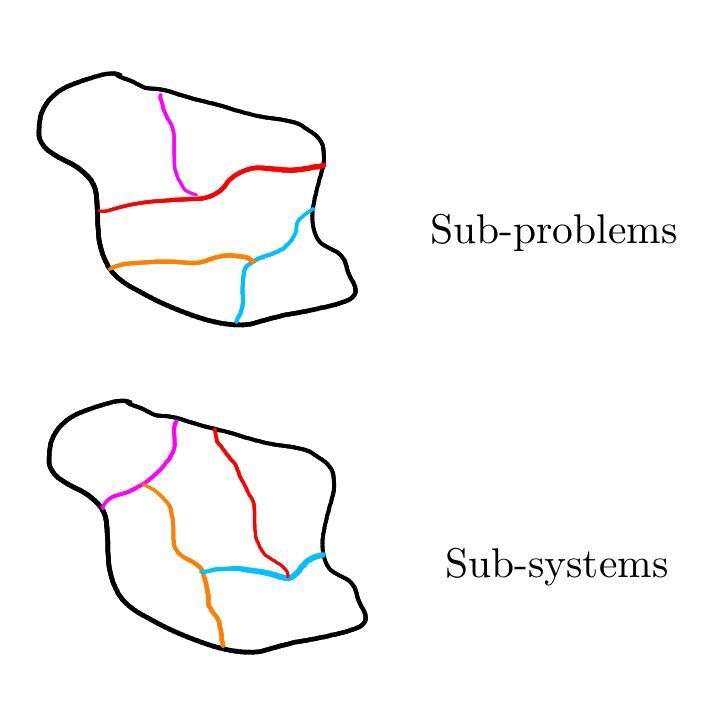
\includegraphics[width=\textwidth,clip,trim=0cm 0 0 2.5cm]{../img/noncorresponding_system_problem.png}
    \caption{Non-correspondending.}\label{fig:noncorresponding_division_system_problem}
  \end{subfigure} \hfill
  \begin{subfigure}{.4\textwidth} \centering
    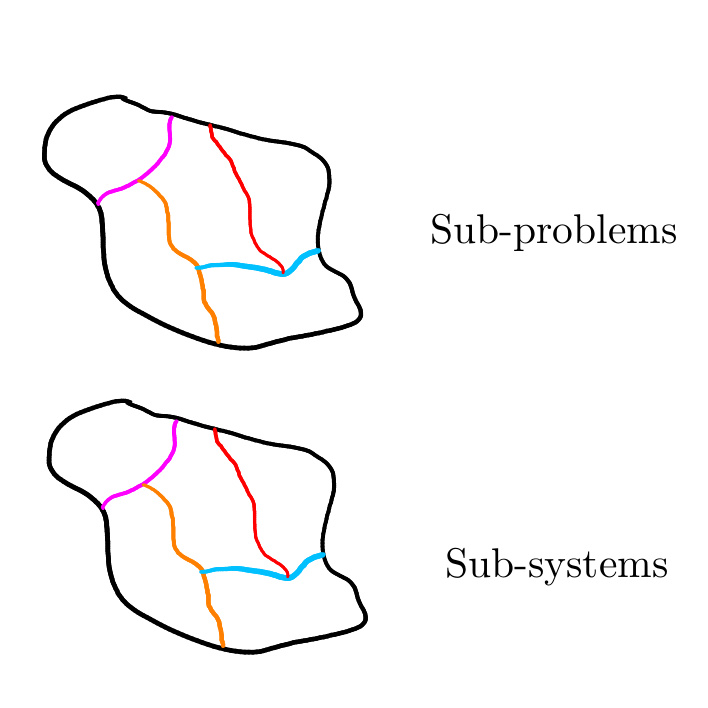
\includegraphics[width=\textwidth,clip,trim=0cm 0 0 2.5cm]{../img/corresponding_system_problem.png}
    \caption{Correspondending.}\label{fig:corresponding_division_system_problem}
  \end{subfigure}
  \caption{Correspondence between decompositions of sub-problems and
    sub-systems.\todo[improve image, add nodes]{}}
\end{figure}

In the literature, it is not unusual to assume that we can choose the computing units in order to correspond to the sub-systems of the system as in Fig.~\ref{fig:corresponding_division_system_problem} (\todo[give examples of units]{Citation?}), i.e., a computing unit computes the solution of a sub-problem to find the input of a corresponding sub-system.
So, in this work we also use this assumption.
Then, the terms sub-problems, sub-systems and agents can be used interchangeably.

\subsection{Do the computing units communicate?}

As shown in the last section (\S~\ref{sec:decomposable_problems}), the only case where communication is not needed to solve the optimization problem is in the uncoupled case (\S~\ref{sec:uncoupled_problems}).
However, there are some decomposition methods for the \dmpc\ that even with coupled problems, they exploit the robustness properties of the MPC to compute the solution without communication~\cite{VahidNaghaviEtAl2014}.
For the decomposition of some optimization problems, it is shown that in certain circumstances the communication is not necessary~\cite{VoulgarisElia2022}.

\begin{remark}
  Usually in \dmpc\ literature the term «decentralized» refers to frameworks where the agents do not communicate~\cite[\S 4]{ChristofidesEtAl2013},\cite{NegenbornMaestre2014}.
  The term can sometimes be confusing and be used even if the agents coordinate themselves.
  In this work we propose a different nomenclature, calling those kinds of frameworks as «uncoordinated control», since there is no coordination between agents nor a coordinator agent to referee. We use the term decentralized as opposed to centralized (monolithic), i.e. to describe structure instead of communication.
\end{remark}

The most part of the literature uses \emph{coordinated control}~\cite{NegenbornMaestre2014, ArauzEtAl2021}, in this work, analogously, we will use a decomposition method where the agents need to communicate.


\subsection{How do the computing units communicate?}

Multiple communication schemes exist, which depend on the decomposition, topology and also trust/power.
We can divide these schemes into two big groups (Fig.~\ref{fig:hierarchic_anarchic}), one where groups of agents are more important than others (\emph{hierarchy}), and another where there is not (\emph{anarchy}).

\begin{figure}[t]
\begin{subfigure}{.45\textwidth}
  \centering
  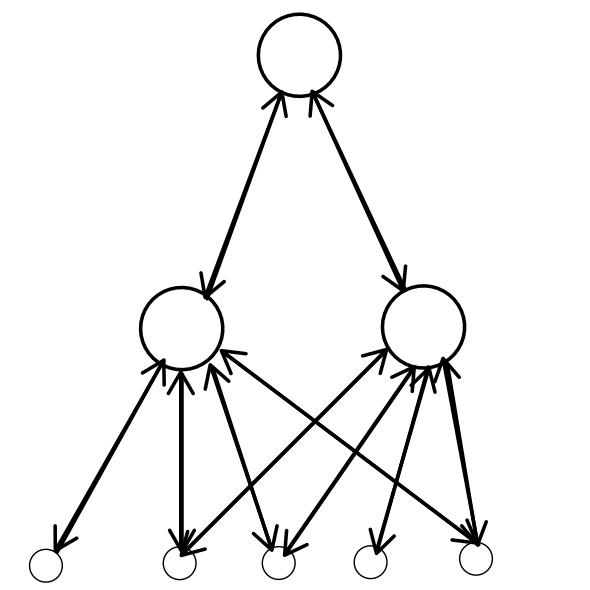
\includegraphics[height=.5\textwidth]{../img/hierarchy.png}
  \caption{Hierarchy.}\label{fig:hierarchy_topology}
\end{subfigure}
\hfill
\begin{subfigure}{.45\textwidth}
  \centering
  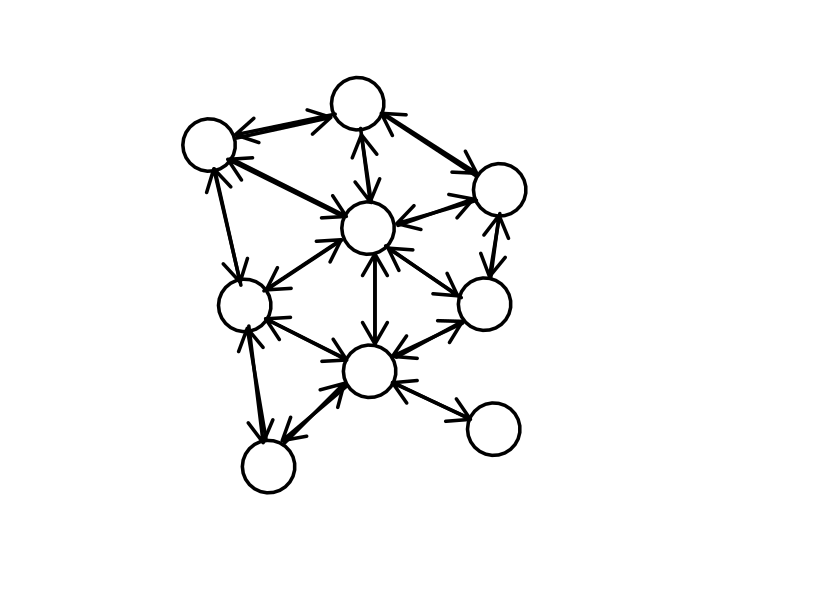
\includegraphics[height=.5\textwidth]{../img/anarchy.png}
  \caption{Anarchy}\label{fig:anarchy_topology}
\end{subfigure}
\caption{Hierarchic and anarchic topologies.}\label{fig:hierarchic_anarchic}
\end{figure}


Sometimes the hierarchical structure may be implied by the decomposition. For instance, some decompositions (\todo[exemplos de sequential dado em ChristofidesEtAl2013]{Citation?}) need the agents to solve their problems one after the other until the values converge (Fig.~\ref{fig:sequential_topology}).
These schemes are called \emph{sequential}.
We can see a hierarchy among the agents, since although a convergence is reached, one group of agents solve their problems disregard the others, giving them an initial position of power, even if temporary.
In other decompositions (\todo[exemplos de parallel dado em ChristofidesEtAl2013]{Citation?}), all agents solve their problems independently of others and then share results until convergence is reached, iteratively or not (Fig.~\ref{fig:parallel_topology}).
These structures are called \emph{parallel}.
In such structures there is no hierarchy.


\begin{figure}[h]
\begin{subfigure}[b]{.45\textwidth}
  \centering
  \begin{tikzpicture}[node distance=1cm and .5cm]
    \node[draw,circle] (first) at (0,0) {};
    \node[draw,circle,right=of first] (second) {};
    \node[draw,circle,right=of second] (third) {};
    \node[draw,circle,opacity=0,right=of third] (fourth) {};
    \node[draw,circle,right=of fourth] (fifth) {};

    \node[] at (fourth) {...};
    \draw[-latex] (first) -- (second);
    \draw[-latex] (second) -- (third);
    \draw[-latex] (third) -- (fourth);
    \draw[-latex] (fourth) -- (fifth);
  \end{tikzpicture}
  \caption{Sequential topology.}\label{fig:sequential_topology}
\end{subfigure}
\hfill
\begin{subfigure}[b]{.45\textwidth}
  \centering
  \begin{tikzpicture}[node distance=.5cm and .5cm]
    \node[draw,rectangle,fill=black,minimum height=2pt,minimum width=5cm] (bar) at (0,0) {};
    % \draw[blue,fill] ($(bar)+(-2.5cm,-2pt)$) rectangle ($(bar)+(2.5cm,2pt)$);
    \node[draw,circle,below=of bar] (third) {};
    \node[draw,circle,left=of third] (second) {};
    \node[draw,circle,left=of second] (first) {};
    \node[draw,circle,opacity=0,right=of third] (fourth) {};
    \node[draw,circle,right=of fourth] (fifth) {};

    \node[] at (fourth) {...};
    \draw[latex-latex]  (first)  -- (bar.south -| first);
    \draw[latex-latex]  (second) -- (bar.south -| second);
    \draw[latex-latex]  (third)  -- (bar.south -| third);
    \draw[latex-latex]  (fifth)  -- (bar.south -| fifth);
  \end{tikzpicture}
  \caption{Parallel topology.}\label{fig:parallel_topology}
\end{subfigure}
\caption{Sequential and parallel topologies.}\label{fig:sequential_parallel_topology}
\end{figure}

And in other decompositions the hierarchical structure can be chosen.
For example, when negotiation between agents is needed, questions about trust and security can shape the presence or absence of hierarchy.
One of these questions is: Can an agent trust all other agents?

This question is common in multiple areas where communication, exchanges or consensus between a large number of agents are needed (politics, economy, and others).
If an agent distrusts the others, it can treat itself the security issues or the agent can outsource the treatment to another agent.
Additional agents can be included to serve as referees, coordinators, regulators or certifiers. It is done because it is easier to trust/verify in a single agent or small group of agents than to trust all agents. The work is divided into more manageable parts.

One real life example can be the \EFT\ between a seller and client. A seller instead of trusting the credit (capacity of paying in future date) of each of its clients, she or he trusts in a small group of credit card brands to fulfill the \EFT{}.
Each credit card brand, in turn, trusts in a select group of credit-granting institutions, to which potentially these client are associated.
This kind of arrangement creates a hierarchical tree-like structure called \emph{polytree} in graph theory terms (Fig.~\ref{fig:polytree_topology}). Seller and clients are leafs (terminal nodes), credit card-brands are branch vertex (intermediary) and the credit-granting institutions are roots (no parent nodes).
Some other political/societal parallel views are stablished in~\cite{McNamaraEtAl2018} and~\cite{OlaruEtAl2018}.

\begin{figure}[h]
  \centering
  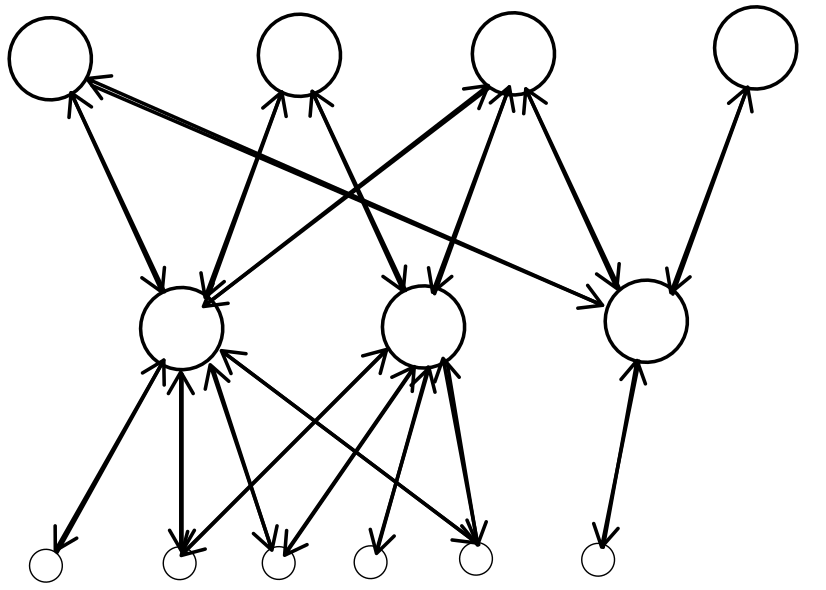
\includegraphics[width=.4\textwidth]{../img/polytree.png}
  \caption{A polytree.\todo[improve figure]{}}\label{fig:polytree_topology}
\end{figure}

\subsubsection{Some drawbacks and compromises}\label{sec:drawbacks}

\paragraph{Failure}
Although the hierarchical structure can help reducing the sources of distrust, it also reduce responsitivity and robustness.
If a small number of the intermediary or most highly nodes in the hierarchical tree are inoperative, there is a possibility that the complete system collapses since the communications will not be accomplished, this problem is commonly known as the \emph{single point of failure}, which can be deviated by the use of redundancy.
On the other hand, for non-hierarchical structures, the system only perish if the majority of the nodes inoperative or compromised.

\paragraph{Energy consumption and Environment}
To overcome the problem of trust in anarchic (peer-to-peer) structures, a solution recently in vogue called \emph{blockchain} was proposed~\todo[add blockchain citation]{Citation ??}.
% The strategy targets exchange of validable data that dependend on historic data.
In this solution, all historic data (log) are shared between all agents.
Before beeing sent to all other agents (or only neighbours), new data need to be processed to generate a \emph{proof of work} (proof of a difficult computation which is easy to test) to create a block.
This block needs to be validated (data and \emph{proof of work} are valid) by at least more than half of the agents before beeing chained into the historic data, forming a chain of blocks, thus the name.

As each block has a different \emph{proof of work}, to create an new block with unreasonable data, a bad ill-intentioned agent needs to alter all the past blocks in the chain recreating all \emph{proof of work} one by one, until the false data could be accepted.
This way, the attacker would need to have more than half of the total processing power of the network.
The \emph{proof of work} strategy trades trust by energy.
A recent work~\cite{ColeCheng2018} estimates the energy consumption of one of the most diffused application of the \emph{blockchain}, a crypto-currency called Bitcoin, being at least $200$kWh for each transaction, which is greater than the monthly electrical consumption of a small household of two people in Brazil~\todo[add BEN]{Citation ??}.
A more recent work~\cite{RoeckDrennen2022} makes a Life Cycle Assessment of Bitcoin mining in a power plant and concludes that its annual emissions of metric tons of CO$_2$-eq is comparable to the annual emissions of 140,000 passenger vehicles.

% \subsection{Conclusion}
All the points above and many others must be considered before choosing a structure.
\todo[some??]{Some} works in the literature of \dmpc\ \cite{VelardeEtAl2017a, BoemEtAl2020, LiuEtAl2022} use an anarchic structure.
Although some methods shown in this work could be adapted to function in analogous structures, we opt to use the hierarchical approach instead. We add coordinator(s) which referee the exchange between agents.

\printbibliography
\end{document}
